\documentclass[12pt,sort&compress]{elsarticle}
\usepackage[utf8]{inputenc}

\newcommand\hmmax{0}
\newcommand\bmmax{0}
\usepackage{bm}
\usepackage{placeins}

\usepackage{mathrsfs}
\usepackage{amsmath}
\usepackage{amsfonts}
\usepackage{amsthm}
\usepackage{upgreek}
\usepackage{color}
\usepackage{sansmath}

\usepackage{array}
%\Meric
%\usepackage{floatrow}

\usepackage{floatrow} % Import floatrow package for customizing float layout
% Set caption position to 'above' for tables
\floatsetup[table]{capposition=top}

\usepackage{graphicx}
\usepackage[tableposition=top]{caption}
%\%%%

\def\bibsection{\section*{References}}

%\iffalse%%%%%%%%%%%%%%%%%%%%%%%%%%%%%%%%%%%%%%
\usepackage{caption}
\captionsetup[figure]{name=Fig.,labelsep=period}

\usepackage{subcaption}
%\fi%%%%%%%%%%%%%%%%%%%%%%%%%%%%%%%%%%%%%%%%%%%
\usepackage{float}
\usepackage{url}
\usepackage{multicol}
\usepackage[top=1in,bottom=1in,left=1in,right=1in]{geometry}
\usepackage[pdfborder={0 0 0},colorlinks,allcolors=blue]{hyperref}
%\usepackage[pdfborder={0 0 0}]{hyperref}
%\usepackage{subfigure}
\usepackage{txfonts}
\usepackage{setspace}
\usepackage{arydshln}
\usepackage{enumitem}
\usepackage{lipsum}% for dummy text
\usepackage{siunitx,booktabs}
\usepackage{nth}
\usepackage{accents} % Accents: circle

\usepackage{float}  % Required for 'H' specifier
\usepackage{floatrow} 

\theoremstyle{definition}%plain/definition/remark
\newtheorem{remark}{Remark}%[section]

% set the graphics path to figures_small or figures_large
%\graphicspath{{figures/}}

%\doublespacing
\onehalfspacing

% prevent overfull boxes...
\sloppy 

% break the equations to avoid white space
\allowdisplaybreaks

\urlstyle{same}

% command for exponents in scientific notation (usage: $1 \times 10^2$ <=> 1\e{2})
\providecommand{\e}[1]{\ensuremath{\times 10^{#1}}}

\newcommand{\etal}{\textit{et al}. }


\usepackage{prettyref}
\newrefformat{fig}{Figure~\ref{#1}}
\newrefformat{Fig}{Fig.~\ref{#1}}
\newrefformat{Eq}{Eq.(\ref{#1})}
\newrefformat{eq}{Eq.(\ref{#1})}
\newrefformat{sec}{Section~\ref{#1}}
\newrefformat{tab}{Table~\ref{#1}}
\newrefformat{Tab}{Table~\ref{#1}}
\newrefformat{alg}{Algorithm~\ref{#1}}
\newrefformat{Alg}{Algorithm~\ref{#1}}

\usepackage[dvipsnames]{xcolor}
\newcommand\hl[1]{%
	\bgroup
	%\hskip0pt\color{red!0!black}%
	\hskip0pt\color{red!80!black}%
	#1%
	\egroup
}

\newtheorem{definition}{Definition}


%======================================== For algorithm
\usepackage{algorithm}
%\usepackage[noend]{algpseudocode}
\usepackage{algpseudocode}
\usepackage{algorithmicx}
\definecolor{shadecolor}{cmyk}{0,0,0,0.03}


\newcommand*\Let[2]{\State #1 $\gets$ #2}
\newcommand*\pnl{\Statex$\vartriangleright$ }
\newcommand*\qpnl{\Statex\quad$\vartriangleright$ }
\newcommand*\qqpnl{\Statex\qquad$\vartriangleright$ }
\newcommand*\qqqpnl{\Statex\quad\qquad$\vartriangleright$ }

\newcommand*\subr[1]{\Statex\textbf{#1}}
\newcommand*\qcomnt[1]{\Statex \textit{#1}}
\newcommand*\qqcomnt[1]{\Statex\quad~~~\textit{#1}}
\renewcommand{\For}[3]{\Statex \textbf{for} \textit{#1} $\leftarrow$ \textit{#2} \textbf{to} \textit{#3} \textbf{do}}
\renewcommand*\EndFor{\Statex \textbf{end for}}

\newcommand*\qFor[3]{\Statex\quad\textbf{for} \textit{#1} $\leftarrow$ \textit{#2} \textbf{to} \textit{#3} \textbf{do}}
\newcommand*\EndqFor{\Statex\quad \textbf{end for}}

\newcommand*\qqFor[3]{\Statex\quad\quad\textbf{for} \textit{#1} $\leftarrow$ \textit{#2} \textbf{to} \textit{#3} \textbf{do}}
\newcommand*\EndqqFor{\Statex\quad\quad \textbf{end for}}

\renewcommand{\If}[3]{\Statex \textbf{if} $#1 #2 #3$ \textbf{then}}
\renewcommand*\EndIf{\Statex\, \textbf{end if}}

\newcommand*\qIf[3]{\Statex\quad\textbf{if} $#1 #2 #3$ \textbf{then}}
\newcommand*\qelse{\Statex\quad\textbf{else}}
\newcommand*\EndqIf{\Statex\quad\textbf{end if}}

\newcommand*\qqIf[3]{\Statex\quad\quad\textbf{if} $#1 #2 #3$ \textbf{then}}
\newcommand*\EndqqIf{\Statex\quad\quad\textbf{end if}}
%=======================================================

%% 
%% Copyright 2007-2020 Elsevier Ltd
%% 
%% This file is part of the 'Elsarticle Bundle'.
%% ---------------------------------------------
%% 
%% It may be distributed under the conditions of the LaTeX Project Public
%% License, either version 1.2 of this license or (at your option) any
%% later version.  The latest version of this license is in
%%    http://www.latex-project.org/lppl.txt
%% and version 1.2 or later is part of all distributions of LaTeX
%% version 1999/12/01 or later.
%% 
%% The list of all files belonging to the 'Elsarticle Bundle' is
%% given in the file `manifest.txt'.
%% 
%% Template article for Elsevier's document class `elsarticle'
%% with harvard style bibliographic references

%% Use the option review to obtain double line spacing
%% \documentclass[preprint,review,12pt]{elsarticle}

%% Use the options 1p,twocolumn; 3p; 3p,twocolumn; 5p; or 5p,twocolumn
%% for a journal layout:
%% \documentclass[final,1p,times]{elsarticle}
%% \documentclass[final,1p,times,twocolumn]{elsarticle}
%% \documentclass[final,3p,times]{elsarticle}
%% \documentclass[final,3p,times,twocolumn]{elsarticle}
%% \documentclass[final,5p,times]{elsarticle}
%% \documentclass[final,5p,times,twocolumn]{elsarticle}

%% For including figures, graphicx.sty has been loaded in
%% elsarticle.cls. If you prefer to use the old commands
%% please give \usepackage{epsfig}

%% The amssymb package provides various useful mathematical symbols
\usepackage{amssymb}
%% The amsthm package provides extended theorem environments
%% \usepackage{amsthm}

%% The lineno packages adds line numbers. Start line numbering with
%% \begin{linenumbers}, end it with \end{linenumbers}. Or switch it on
%% for the whole article with \linenumbers.
 \usepackage{lineno}

% ---- PRINT HIGHLIGHTS IN PDF (local preview only) ----
\usepackage{enumitem}
\makeatletter
\renewenvironment{highlights}
  {\section*{Highlights}\begin{itemize}[leftmargin=*,noitemsep,topsep=0pt]}
  {\end{itemize}}
\makeatother
% ------------------------------------------------------
\linenumbers
\journal{TBD}

\begin{document}
\begin{frontmatter}

%% Title, authors and addresses

%% use the tnoteref command within \title for footnotes;
%% use the tnotetext command for theassociated footnote;
%% use the fnref command within \author or \address for footnotes;
%% use the fntext command for theassociated footnote;
%% use the corref command within \author for corresponding author footnotes;
%% use the cortext command for theassociated footnote;
%% use the ead command for the email address,
%% and the form \ead[url] for the home page:
%% \title{Title\tnoteref{label1}}
%% \tnotetext[label1]{}
%% \author{Name\corref{cor1}\fnref{label2}}
%% \ead{email address}
%% \ead[url]{home page}
%% \fntext[label2]{}
%% \cortext[cor1]{}
%% \affiliation{organization={},
%%             addressline={},
%%             city={},
%%             postcode={},
%%             state={},
%%             country={}}
%% \fntext[label3]{}

%\title{Large-Eddy Simulation of the Piscataqua River: A Feasibility Analysis for deployment of a Tidal Site Under Ebb and Flood Conditions}
\title{Comparative Analysis of ADCP Data Used in CFD Simulations}

\author[sbu]{Jonathan Craig}
\author[sbu]{Hossein Seyedzadeh}
\author[sbu]{Ali Khosronejad\corref{cor1}}
\ead{}
\cortext[cor1]{Corresponding author}
\address[sbu]{Department of Civil Engineering, Stony Brook University, Stony Brook, NY 11794, USA}

\begin{abstract}

\noindent .
\end{abstract}

\begin{keyword}
{Marine hydrokinetic turbine; Utility-scale tidal farms; Acoustic Doppler Current Profiler; Turbulent Flow}
\end{keyword}

\end{frontmatter}
\clearpage   % or \newpage
\iffalse
\begin{highlights}
\item F.
\item M.
\item R.
\item S.
\item A.
\end{highlights}
\fi

\section{Introduction}
\label{sec:intro}

\noindent In modern efforts to further renewable energy through research and application, it is essential to quantify the theoretical, technical, and practical as defined by the International Electrotechnical Commission \cite{iea_2020}. Renewable energy research is exploring yet untapped sources such as marine energy which comprises waves, tides, and currents. As of 2021, the National Laboratory of the Rockies (NLR) reported that the United States encompass 2300 TWh/yr in total of extractable marine energy, with 830 TWh/yr of extractable marine energy from the contiguous US alone \cite{nrel_2021}. Even though total energy consumption in 2024 was equal to 26,349.45 TWh/yr, the total technical resource can theoretically provide more than enough power for all the households in the USA (please refer to \autoref{tab:data_summary}). Another consideration for marine energy industry is energy policy whether sponsored by the federal government or by state governments. Through the bipartisan coalition known as Clean Energy States Alliance (CESA),  more than 20 states aim for a transition to 100\% clean energy by 2050 \cite{cesa}; however, only few states such as Maine explicitly name marine renewable energy (MRE) in their summaries of utility-scale renewable energy sources \cite{cesa}. Even without consideration of rivers, MRE is geographically accessible through waves and tidal currents that occur in 23 of the 50 states \cite{nrel_2021}. Tidal currents constitute an especially potent, predictable energy resource with relatively low variation by weather in comparison to wind and solar, as well as likely negligible environmental impact in comparison to traditional hydropower such as dams and barrages \cite{Legrand-2009-1509, [osalusi_2009], [ouro_2019], nrel_2021, [lieber_2024],  [keenan_2024]}. This energy resource is accessible through the introduction of marine hydrokinetic (MHK) turbines that are installed in the tidal or riverine current to generate electricity without major obstruction of the tides. 

A key step to marine technologies' consistent adoption and operation between countries is the development of technical standards such as the International Electrical Commission Technical Specification (IEC TS) 62600-21 for the assessment and characterization of tidal energy resources. As in similar studies about wind energy \cite{[mccaffrey_2015],[naberezhnykh_2023]}, the IEC TS could serve as guidelines between various studies so that they could explore or validate information about tidal technologies within the same parameters for comparison throughout studies as well as participating countries \cite{kilcher_tidal_2023,[deb_2025],[naberezhnykh_2023],[lieber_2024],[mcvey_2026]}. Even though some studies reported varied degrees of discrepancies between recommended guidelines, \cite{[mccaffrey_2015],[naberezhnykh_2023],[lieber_2024]}, the recent version-namely, the IEC TS 62600-21-stands as an opportunity to explore the updated standards' applicability. Within Table 1 of IEC TS 62600-201, Stages 1 and 2 likely correspond to the technical and practical resources defined by \citet{iea_2020} and outlined by \citet{nrel_2021}. The first stage entails a general feasibility study of the complete relevant environment. The next stage is concentrated on the TEC array design at the deployment site. 

\iffalse
This analysis intends to explore the transition between these two stages. As stated in the methodology within Section 5.2 of the IEC TS 62600-201, one may compute AEP either from in-field data or from hydrodynamic modeling. 
\fi

Industrial interest for tidal turbines' deployment can concern the transition between stages 1 and 2, which entails in-field data collection \cite{[gooch_2009]}. Some models had inaccurately predicted tidal energy sites' power density \cite{kilcher_tidal_2023}. Since power generated is proportional to the cube of fluid velocity, accurate data collection and modeling is critical to MHK turbines' simulation before deployment \cite{[korotenko_2019]}. Notwithstanding the tidal cycles' predictability by deacdes into the future, the highly energetic turbulence that characterizes tidal environments reinforces the need for accurate in-situ data collection to predict power generation as well as other parameters such as MHK turbines' structural performance over their lifetimes \cite{[deb_2025], lieber_2024], [greenwood_2019],[neary_2011]}. Likewise, riverine environments exhibit more variable discharge, depth, and turbulence in spite of their assumed unidirectional flow \cite{[neary_2011]}. Technologies including acoustic Doppler current profilers (ADCPs) and acoustic Doppler velocimetry (ADV) serve as common data collection methods from sites and experiments to characterize sites for bathymetry and inflow conditions in computational fluid dynamic (CFD) simulations \cite{[gargett_1994], [levine_2009], [gooch_2009], [thomson_2010], [stevens_2012], [thomson_2012], [mycek_2014],[guion_2014], [korotenko_2019], [ouro_2019], [keenan_2024], [karsten_2024], deb_2025], [mcvey_2026]}. In-field measurements from ADCP alone do not supply enough data for a site's complete 3D hydrodynamic behavior. Hence, the IEC framework advises hydrodynamic modeling to refine flow characterization, energy estimation, and uncertainty quantification when the annual energy production (AEP) reaches higher than 2\% of the theoretical tidal energy resource\cite{noauthor_iec_nodate}. In Table 1 of the IEC TS 62600-201, the Stage 2 resource assessment emphasizes the need for detailed turbulence statistics, including turbulence intensity, turbulence kinetic energy (TKE), Reynolds stresses, vertical shear, and wake interactions, all of which can significantly affect turbine loading, fatigue behavior, wake recovery, and overall farm performance \cite{noauthor_iec_nodate}.


%Following the Princeton Ocean Model proposed by Blumberg and Mellor (1987), Chen et al. (2006) launched the Finite-Volume Coastal Ocean circulation Model (FVCOM) for more accurate digital modeling of complex bathymetry and shorelines. Its hallmark is the solution of the flux form of the 3D hydrostatic primitive equations within an unstructured triangular meshing for better matching between physical and digital coasts with diverse forcing from tides, wind, and river discharge  [chen2006]. Following a recent field survey by McVey and Kilcher, Deb et al. (2025) advocated 3D coastal models such as FVCOM and Mellor-Yamada Level 2.5 Turbulence Model to provide boundary conditions macro-scale turbulence for tidal farm layout design as per Stage 2 of the IEC.

\iffalse
This report documents the preprocessing of tidal current data from the Center for Operational Oceanographic Products and Services (CO-OPS) of the National Oceanic and Atmospheric Administration (NOAA) for CFD analysis. CFD takes place by LES with the in-house Virtual Flow Simulator (VFS) software \cite{MHKDR_Dataset_496} for the Long Island Sound Tidal Energy Project report of Verdant Power. This article aims to serve as an example to the transition between Stages 1 and 2 in Table 1 of the IEC TS 62600-201. 
\fi

In this study, a new workflow based on the report of \citet{husoVP2026} processes ADCP measurements from the Center for Operational Oceanographic Products and Services (CO-OPS) of the National Oceanic and Atmospheric Administration (NOAA) within Python for future high-fidelity CFD simulations. It is essentially a demonstration of the transition between Stages 1 and 2 in Table 1 of the IEC TS 62600-201 between the respective description of a prospective site's and validation of outputs to serve as CFD inflow conditions. Consistent with the recommendations of IEC TS 62600-201 \cite{noauthor_iec_nodate} for Stage 2 resource assessment, the present study focuses on the characterization of mean flow properties, turbulence variability, and directional hydrodynamic asymmetry between ebb and flood tides. The processed ADCP data and resource characterization presented herein will support the development, calibration, and validation of future LES models incorporating realistic bathymetry, turbine-array interactions, turbulence-resolving flow physics, and farm-scale hydrodynamics for utility-scale marine energy applications in Long Island Sound.

=======
\iffalse
Accurate tidal resource assessment is essential for the successful development and deployment of marine energy systems. According to IEC TS 62600-201, hydrodynamic modeling plays a critical role in tidal resource characterization because tidal flows are inherently complex, spatially variable, and strongly influenced by turbulence, bathymetry, coastline geometry, and directional asymmetry between ebb and flood tides. While field measurements such as ADCP data provide valuable site-specific observations, measurements alone are often insufficient to fully characterize the three-dimensional hydrodynamic behavior required for engineering-scale resource assessment and turbine-array design. For cases in which the Annual Energy Production (AEP) exceeds approximately 2\% of the theoretical tidal energy resource, the IEC framework recommends the use of hydrodynamic modeling to improve the accuracy of flow characterization, energy estimation, and uncertainty quantification. In particular, Stage 2 resource assessment emphasizes the need for detailed turbulence statistics, including turbulence intensity, turbulence kinetic energy (TKE), Reynolds stresses, vertical shear, and wake interactions, all of which can significantly affect turbine loading, fatigue behavior, wake recovery, and overall farm performance \cite{noauthor_iec_nodate}.

In this study, a new workflow processes ADCP measurements from CO-OPS within Python to characterize the hydrodynamic conditions at a prospective tidal energy site in the Long Island Sound, and to provide the required input and validation data for future high-fidelity CFD simulations. This work represents a key transition from the feasibility assessment to the array design of a broader modeling framework for high-resolution LES of tidal turbine subhub arrays under realistic environmental conditions. Consistent with the recommendations of IEC TS 62600-201 \cite{noauthor_iec_nodate} for Stage 2 resource assessment, the present study focuses on the characterization of mean flow properties, turbulence variability, and directional hydrodynamic asymmetry between ebb and flood tides. The processed ADCP data and resource characterization presented herein will support the development, calibration, and validation of future LES models incorporating realistic bathymetry, turbine-array interactions, turbulence-resolving flow physics, and farm-scale hydrodynamics for utility-scale marine energy applications in Long Island Sound.
\fi

\section{Methodology}
\label{sec:2}
\subsection{Data collection}
\label{subsec:2.1}
Based on \cite{kilcher_tidal_2023}, Long Island Sound (LIS) is identified as one of the major tidal energy hotspots in the United States, with an estimated tidal power density of approximately 1.2 $kW/m
^2$. Consequently, the present study is focused on a prospective tidal energy site by Orient Point at the eastern end of the LIS. Multiple sources of observational data characterize relevant sites' hydrodynamic conditions \cite{kilcher_tidal_2023, coops_map}. For the study area of the eastern LIS, ADCP measurements are obtained from data in the CO-OPS map interface provided NOAA \cite{coops_map}, along with field sonar measurements provided by Verdant Power which is this study's industrial partner. These datasets informed the tidal flow characteristics with fundamental hydrodynamic data for future high-fidelity numerical modeling and IEC-compliant tidal resource assessment.

\begin{table}[h!]
\centering
\caption{Potential contributions of technical marine energy resources to electricity generation and power to households in the United States of America. Technical marine energy resource data come from \citet{nrel_2021} with updated data of electricity generation and domestic electric consumption from \citet{owid_energy_united_states}, \citet{uscensus_household}, and \citet{eia_electricdomestic}. As of V2025, the total number of households in the USA is 148,260,882.}

\label{tab:data_summary}
\begin{tabular}{lccccc}
\hline
\textbf{Energy} & \textbf{Technical resource [TWh/hr]} & \textbf{Electricity total [\%]} & \textbf{Potential power for households} & \textbf{Households powered [\%]}\\
\hline
Marine total & 2300 & 55 & 210000000 &  \\
Tidal total & 220 & 5.3 & 20000000 &  \\
Tidal in contiguous U.S.A & 15 & 0.36 & 1400000 &  \\
Riverine in contiguous U.S.A & 79 & 1.9 & 73000000 &  \\
\hline
\end{tabular}
\end{table}


\begin{table}[h!]
\centering
\caption{Summary of ADCP and field measurement datasets used for hydrodynamic characterization and tidal resource assessment within the Long Island Sound study area. Verdant Power was responsible for the data collection in the LIS, which \cite{husoVP2026} covered.}
\label{tab:data_summary}
\begin{tabular}{lcccccc}
\hline
\textbf{Site code} & \textbf{Start date (duration) [days]} & \textbf{Record interval [min]} & \textbf{Bin size [m]} & \textbf{Mean depth [m]} & \textbf{Source} \\
\hline
LIS & October 23, 2024 (115) & 10 & 1.67--25.67 (0.5) & -- & Verdant Power \\
RC & Aug 2, 2010 (31) & 6 & 2.7--14.7 (1) & 16.4 & \cite{37} \\
\hline
\end{tabular}
\end{table}

% This will be used later by Jono
%\iffalse
The tidal data originate from the Center for Operational Oceanographic Products and Services (CO-OPS) which is based within NOAA \cite{coops_map}. CO-OPS collects data of tides, currents, water levels, and weather at 200 stations over the coasts and Great Lakes of the USA including Hawai'i and Alaska. Altogether, these data intend to improve navigation safety, to provide guiding data to coastal and hydrographic surveys, and to prepare coastal communities for climate change. Temporary meters record tidal current data for use as historical references. On the CO-OPS website, these predictions visualize necessary data as sinusoidal plots of ebb, flood, and slack accompanied by tabulated values. Plotting options include the time range in hours or weeks, time zone, data interval, units, and choice of date from the website's selection. Furthermore, the prediction plots specify the mean flood and ebb directions relative to true north.

A noticeable constraint is that sites are fixed whereas tidal turbine siting can be more particular and tentative. Even though the sites marked by CO-OPS do not exactly coincide with the desired study area herein, they can serve as benchmarks to guide future in-situ data collection or feasibility studies for IEC Stage 1 analysis. Another caveat is a given site's data range. Only marked sites contain multiple bin data whereas other sites monitor only one depth. Likewise, some sites have months' worth of data whereas others register tidal data only over days' span. Moreover, the CO-OPS website only concatenates one month of tidal data in one file, and so the user must handle any further concatenation between months. For these considerations, the study has selected Cornfield Point which is denoted as LIS1016 in the website. It lies at 4 miles (6.4 km) to the south of Buoy CF which approximates Verdant Power's MHK turbine siting. Also, the timeframe ranges over a month and a half, which is acceptable for this report's tidal analysis and eventual CFD discussion.

For a comprehensive tidal analysis, each depth and month output a CSV file to be downloaded into a folder. Therein, MATLAB source files read the data for supplementary tidal analysis. Since CO-OPS does not distinguish files beyond only the site name, these source files must be manually renamed for clarity and for the intended algorithm in MATLAB. This MATLAB code supplements the tidal analysis and CFD simulations conducted by \citet{husoVP2026}, which are available in GitHub (https://github.com/hosseinsz93/Verdant-SBU-tidal-project). 
%\fi

\subsection{Principal flow direction}
\label{subsec:2.2}

\noindent Tidal currents are generally characterized by dominant ebb and flood phases, which become the channel's principal flow direction when condensed to a single axis. The following formula yields the principal flow axis:

\[
\theta_{\text{principal}}
=
0.5
\arctan^2
\left(
\langle \sin(2\theta)\rangle,
\langle \cos(2\theta)\rangle
\right)
\]

where \(\theta\) denotes the depth bins' average orientation. This formula identifies the dominant, bidirectional tidal flow axis along which the flood and ebb currents run. Since the ebb and flood directions are opposite but parallel, running about \(180^{\circ}\) from each other, this approach collapses the two directions into a single principal flow axis.

\subsection{Velocity profiles}
\label{subsec:2.3}

\noindent Accurate characterization of the inflow velocity profile is essential for hydrodynamic modeling and tidal resource assessment. Field observations commonly employ ADCP collect data about waves, tides, and  currents for marine engineering, hydrodynamic modeling, and resource management \cite{[thomson_2012],[kakarla_2023]}. Nonetheless, the higher Doppler noise in ADCP than ADV often entails that the unprocessed data exhibit a large standard error  \cite{[thomson_2010],[thomson_2012]}. Consequently, theoretical and empirically derived velocity profile formulations are commonly employed to represent depth-dependent flow behavior in turbulent boundary layer flows. 

The von K\'arm\'an--Prandtl logarithmic law and power-law velocity profiles serve as common models for fully developed open-channel flows which can be extended to tidal flows. Previous studies have shown that power-law formulations overall represent tidal current velocity distributions more accurately than the logarithmic law, particularly outside the near-bed region where the assumptions of the log-law formulation are less applicable \cite{jang_current_2026}. Otherwise, the logarithmic law is theoretically valid within the inner region of the turbulent boundary layer near the bed.

The power-law profile can be modified as such to incorporate the effect of bed roughness:

\[
\overline{u}(z)
=
\left(
\frac{z}{\beta h}
\right)^{\frac{1}{\alpha}}
U
\]

where \(\overline{u}(z)\) is the streamwise velocity at elevation \(z\) above the bed \((m/s)\), \(z\) is the height above the bed \((m)\), \(U\) is the depth-averaged velocity \((m/s)\), and \(h\) is the total water depth \((m)\). The parameter \(\alpha\) represents the power-law exponent, while \(\beta\) is the bed roughness coefficient that takes near-bed flow effects into account. The division of $z$ and $h$ can be represented as a normalized vertical coordinate $\eta$ for a nondimensional velocity profile:

\[
\frac{\overline{u}}{U}
=
\left(
\frac{\eta}{\beta}
\right)^{\frac{1}{\alpha}}
\]

Also, the log law can be written as follows:

\[
\overline{u}(z)=
\frac{u_*}{\kappa}
\ln
\left(
\frac{z}{z_0}
\right)
\]
where $\overline{u}(z)$ is the mean streamwise velocity at height $z$, $u_*$ is the friction velocity, $\kappa$ is the von Kármán constant $\approx 0.41$, $z$ is the distance above the bed, and
$z_0$ is the hydrodynamic roughness length.

%%We employed the spatially filtered Navier-Stokes equations for incompressible flow in non-orthogonal generalized curvilinear coordinates. Using compact Newton notation, where repeated indices imply summation, these equations are expressed as follows \cite{[10],[83],[84], [91], [92],[120], AWR_5}:

%%\begin{equation}
%%    J\frac{\partial U^j}{\partial\xi^j}=0
%%    \label{eq:1}
%%\end{equation}

%%\begin{equation}
%%    \frac{1}{J}\frac{\partial U^i}{\partial t}=\frac{\xi_l^i}{J}\left(\frac{\partial}{\partial\xi^j}\left(U^ju_l\right)+\frac{1}{\rho}\frac{\partial}{\partial\xi^j}\left(\mu\frac{g^{jk}}{J}\frac{\partial u_l}{\partial\xi^k}\right)-\frac{1}{\rho}\frac{\partial}{\partial\xi^j}\left(\frac{\xi_l^jp}{J}\right)-\frac{1}{\rho}\frac{\partial\tau_{lj}}{\partial\xi^j}+F_{\mathrm{ext}}\right)
%%    \label{eq:2}
%%\end{equation}

%%\noindent where $J = \left| \partial(\xi^1, \xi^2, \xi^3)/\partial(x_1, x_2, x_3) \right|$ is the Jacobian of geometric transformation, which handles the transformation from the Cartesian coordinate system to the curvilinear system. The contravariant volume flux is expressed as $U^i = (\xi_l^i/J) u_l$, where $\xi_l^i = \partial \xi^i/\partial x_l$. The contravariant metric tensor is given by $G^{jk} = \xi_l^j \xi_l^k$. $u_i$ denotes the $i$-th filtered velocity component in the Cartesian coordinate system. $p$ represents the pressure term, and $\rho$ is the density of the river water and set equal to $1000$ $kg/m^3$. $F_{\mathrm{ext}}$ represents the lift and drag forces' contribution per unit volume to the momentum equations as source terms. The subgrid-scale stresses in the LES turbulence model are captured using the dynamic Smagorinsky model and are defined as follows
%% \cite{kevin_uncertainity, [70], [69]}:

%%\begin{equation}
%%     \tau_{lj}=-2\mu_{\mathrm{t}} \overline{S}_{lj}+\frac{1}{3}\tau_{kk}\delta_{lj} 
%%    \label{eq:3}
%%\end{equation}
%%\begin{equation}
%%    \mu_{\mathrm{t}} = C_{\mathrm{s}}\Delta^2 \left |\overline{S} \right|
%%    \label{eq:4}
%%\end{equation}

%%\begin{equation}
%%\left |\overline{S} \right| = \sqrt{2 (\overline{S_{lj}} \overline{S_{lj}} )}
%%\label{eq:5}
%%\end{equation}

%%\noindent where $\mu_{\mathrm{t}}$ represents the eddy viscosity, $\overline{S}_{ij}$ denotes the filtered strain-rate tensor, and \( \delta_{ij} \) is the Kronecker delta. $C_\mathrm{s}$ shows the Smagorinsky constant, and filter size is $\Delta = J^{-1/3}$ with volume of the cell shown as $J$ \cite{kevin_uncertainity, [120]}.

%%\subsection{Turbine Modeling}

%%\begin{equation}
%%  F_{\mathrm{D}}=\frac{1}{2}c\rho C_{\mathrm{D}}V_{\mathrm{rel}}^2
%%  \label{eq:6}
%%\end{equation}
%%\begin{equation}
%%   F_{\mathrm{L}}=\frac{1}{2}c\rho C_{\mathrm{L}}V_{\mathrm{rel}}^2
%%   \label{eq:7}
%%\end{equation}


%%\noindent where $c$ denotes the chord length of the turbine blade. The drag and lift coefficients, $C_{\mathrm{D}}$ and $C_{\mathrm{L}}$, respectively, are functions of the Reynolds number and the angle of attack \cite{[55]}. Additionally, a detailed explanation of the tip loss effects and the resulting corrected drag and lift coefficients can be found in \cite{[55]}.
%%The relative velocity, $V_{\mathrm{rel}}$, is defined as follows \cite{[76],[119]}:

%%\begin{equation}
%%V_{\mathrm{rel}} = \left(u_x, u_\theta - \Omega r\right)
%%\label{eq:8}
%%\end{equation}

%%\noindent where $\Omega$ denotes the angular velocity of the rotor, and $r$ is the distance of each segment along the actuator line from the rotor center. The terms $u_x$ and $u_\theta$ represent the velocity components averaged over the actuator line in the axial and azimuthal directions, respectively, and are defined as follows \cite{[76]}:

%%\begin{equation}
%%u_x = \mathbf{\bm{u}}\left(X\right) \cdot \mathbf{\bm{e}}_x
%%\label{eq:9}
%%\end{equation}

%%\begin{equation}
%%u_\theta = \mathbf{\bm{u}}\left(X\right) \cdot \mathbf{\bm{e}}_\theta
%%\label{eq:10}
%%\end{equation}

%%\noindent where $\mathbf{\bm{e}}_x$ and $\mathbf{\bm{e}}_\theta$ denote the unit vectors respectively in the axial and azimuthal directions. The terms $x_i$ and $X_i$, with $i = 1, 2, 3$ in compact tensor notation, represent the Cartesian and Lagrangian coordinate systems, corresponding to the fluid grid nodes and actuator lines.
%%The velocity at the actuator line points is interpolated from the background grid nodes using a discrete delta function, $\delta_h$, defined as follows \cite{[76],[77]}:


%%\begin{equation}
%%\mathbf{\bm{u}}(X) = \sum_{N_f} \mathbf{\bm{u}}(\mathbf{\bm{x}}) \delta_h(x - X) V(x)
%%\label{eq:11}
%%\end{equation}

%%\begin{equation}
%%\delta_h(x-X) = \frac{1}{V} \phi\left(\frac{x-X}{h_x}\right) \phi\left(\frac{y-Y}{h_y}\right) \phi\left(\frac{z-Z}{h_z}\right)
%%\label{eq:12}
%%\end{equation}

%%\noindent where $N_f$ denotes the total number of fluid cells, $V(x)$ represents the volume of each fluid cell \cite{[76]}, and $\phi$ denotes the smoothed four-point cosine function \cite{[55]}

% \begin{equation}
% \phi = -\tan^{-1} \left( \frac{u_x}{u_\theta - \Omega r} \right)
% \label{eq:13}
% \end{equation}

%%Assuming a uniform distribution of force along the chord length, the force per unit area can be expressed as follows \cite{[76]}:

%%\begin{equation}
%%f(X) = \frac{\left(F_{\mathrm{L}} + F_{\mathrm{D}}\right)}{c}
%%\label{eq:14}
%%\end{equation}

%%Once all parameters are obtained from \prettyref{eq:6} to \prettyref{eq:14}, the distributed body force is computed as follows \cite{[76]}:

%%\begin{equation}
%%f_{\mathrm{AL}}(x) = \sum_{N_{\mathrm{f}}} f(X) \delta_h(x-X) A(X)
%%\label{eq:15}
%%\end{equation}

\subsection{Turbulence intensity}
\label{subsec:2.4}

\noindent Characterization of turbulence intensity is an important component of IEC TS 62600-201 Stage 2 tidal resource assessment, as turbulence strongly influences turbine loading, wake recovery, fatigue behavior, and uncertainty in Annual Energy Production (AEP) estimates. However, accurate turbulence measurements in energetic tidal environments remain challenging due to instrument limitations and measurement uncertainty \cite{neill_tidal_2021}.

ADCP measurements inherently contain instrumental noise associated with the estimation of Doppler shifts from finite-length acoustic pulses. This uncertainty is commonly referred to as Doppler noise \cite{curm_1990}. Consequently, turbulence statistics derived directly from ADCP velocity measurements may contain artificial variance contributions unrelated to the physical flow turbulence.

To account for this effect, turbulence intensity calculations were corrected for instrument-induced white noise following methodologies commonly adopted in tidal resource assessment studies \cite{sellar_characterisation_2018}. The corrected streamwise turbulence intensity, \(I_u\), is calculated as:

\[
I_u
=
\frac{
\sqrt{
\sigma_u^2
-
\sigma_{\text{noise}}^2
}
}{
\overline{u}
}
\]

where \(\sigma_u^2\) is the variance of the streamwise velocity fluctuations, \(\sigma_{\text{noise}}^2\) is the variance associated with instrument white noise, and \(\overline{u}\) is the mean streamwise velocity. Turbulence intensity values were computed for each spatial measurement bin within the ADCP profile.

The white-noise variance was estimated using spectral analysis techniques based on the approach proposed in previous studies \cite{sellar_characterisation_2018}. This procedure involves fitting the power spectral density of the velocity fluctuations using a two-component representation consisting of:

\begin{itemize}

\item a turbulent inertial subrange characterized by the Kolmogorov \(f^{-5/3}\) spectral slope, and

\item a frequency-independent white-noise component representing instrumental Doppler noise.

\end{itemize}

This correction procedure improves the reliability of turbulence statistics extracted from ADCP measurements and provides more physically representative estimates of turbulence intensity for hydrodynamic characterization and future high-fidelity CFD and LES model development.

\section{Results and Discussions}
\label{sec:3}
\subsection{ADCP data analysis}
\label{sec:3.1}

\noindent Data collection originated from LIS1016 of CO-OPS. The choice of this study for demonstration was based on its proximity to the site examined by \citet{husoVP2026}. This dataset's deployment period lasted from 20:10:00, Jun 9, 2010 until 18:34:00, Jul 27, 2010, with a collection interval of 6 minutes. Thus, there were a total of 11503 samples were analyzed: 3,356 for ebb and 3,379 for flood. For consistency with \citet{husoVP2026}, the data analysis defined the slack threshold velocity as \(0.4~m/s\). This corresponded to the turbine cut-in velocity which should reduce uncertainty associated with near-slack flow conditions.

Next, the code generated depth-dependent and depth-averaged data frames. These processed datasets were then utilized for subsequent hydrodynamic and tidal resource analyses.

\subsubsection{Principal flow direction}

The principal flow axis was found to run along $63.7^{\circ}$ in the direction of ebb. Unlike to the orientation offset in \citet{husoVP2026}, there was no need to correct the principal flow between ADCP measurements for directional continuity over the full observation period. Both ebb and flood exhibited a small misalignment from the principal flow axis, with ebb at $66.9^{\circ}$ and flood at $61.4^{\circ}$. The observed difference of approximately \(6^{\circ}\) between ebb and flood principal directions indicates a degree of directional asymmetry within the site, likely associated with local bathymetric effects and channel geometry.

The following formula projected velocity components onto the principal flow axis:

\[
u_s = u\cos\theta + v\sin\theta
\]

where \(u_s\) represents the streamwise velocity component aligned with the principal tidal flow direction.

\subsection{Profile shape and classification}
\label{sec:3.2}

\noindent As described earlier in \autoref{subsec:2.3} representative velocity profiles in tidal boundary-layer flows are commonly described using either power-law or logarithmic-law formulations. These analytical profiles are frequently employed in tidal resource assessment and hydrodynamic modeling to characterize the vertical structure of the flow and to provide physically representative inflow conditions for numerical simulations.

Figures~\ref{Fig:logLaw} and ~\ref{Fig:powerLaw} illustrate typical logarithmic and power-law velocity profile shapes commonly observed in turbulent open-channel and tidal flows, respectively. Using the processed ADCP measurements provided by Verdant Power, individual tidal cycles (shown in \autoref{Fig:tidalCycle}) were extracted and analyzed to investigate the vertical velocity structure during both ebb and flood conditions, as shown in Figure~\ref{Fig:tidalCycle}.

\iffalse
Each tidal cycle contains a depth-dependent velocity distribution that can be approximated using either logarithmic-law or power-law formulations. In the present study, the velocity profiles were fitted using the modified power-law formulation introduced previously:

\[
\overline{u}(z)
=
\left(
\frac{z}{\beta h}
\right)^{\frac{1}{\alpha}}
U
\]

where:

\begin{itemize}

\item \(\overline{u}(z)\) is the streamwise velocity \((m/s)\),
\item \(z\) is the elevation above the bed \((m)\),
\item \(U\) is the depth-averaged velocity \((m/s)\),
\item \(h\) is the total water depth \((m)\),
\item \(\alpha\) is the power-law exponent, and
\item \(\beta\) is the bed roughness coefficient.

\end{itemize}
\fi

The fitted velocity profiles obtained from the Verdant Power ADCP measurements are presented in Figure~\ref{Fig:powerLaw}. The resulting fitted parameters are:

\begin{table}[H]
\centering
\caption{H}
\label{tab:comp_det}
\begin{tabular}{cccc}
\hline
\textbf{Tide} & \textbf{$\alpha$} & \textbf{$\beta$} & \textbf{U [m/s]}\\
\hline
Ebb & 3.35 & 0.467 & 1.56 \\
Flood & 4.95 & 0.450 & 1.33 \\
\hline
\end{tabular}
\end{table}

The results indicate slight asymmetry between ebb and flood tidal conditions, reflected in both the fitted power-law exponents and the depth-averaged velocities. Such asymmetry is likely associated with local bathymetric effects, channel geometry, and directional hydrodynamic variability within the study site. These fitted profiles provide important hydrodynamic characterization for IEC-compliant tidal resource assessment and will also be used to support the development of realistic inflow boundary conditions for future high-fidelity LES simulations of turbine-array hydrodynamics in Long Island Sound.

\begin{figure} [H]
  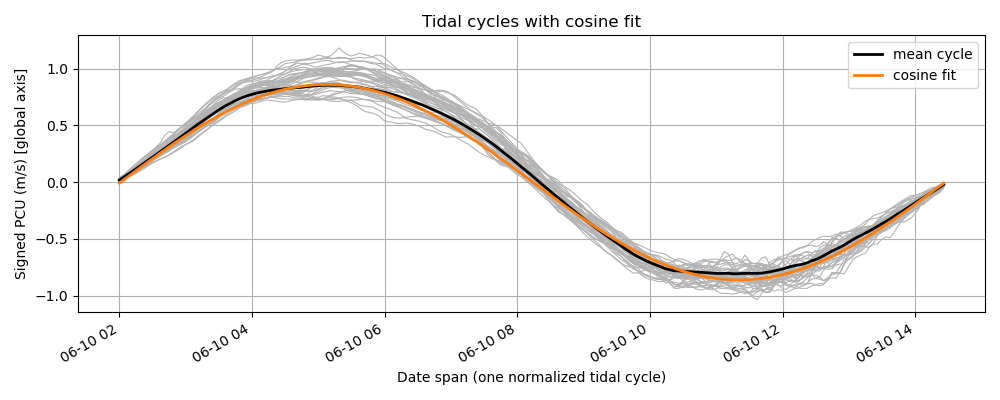
\includegraphics[width=1\textwidth]{./figure/tidalCycle.png} 
  \caption{Tidal cycles extracted from the Verdant Power ADCP measurements together with the corresponding cosine-function fit. Gray lines represent individual normalized tidal cycles, the black line denotes the ensemble-averaged tidal cycle, and the orange curve shows the fitted cosine representation used to characterize the periodic tidal behavior.}
  \label{Fig:tidalCycle}
\end{figure}

\begin{figure} [H]
  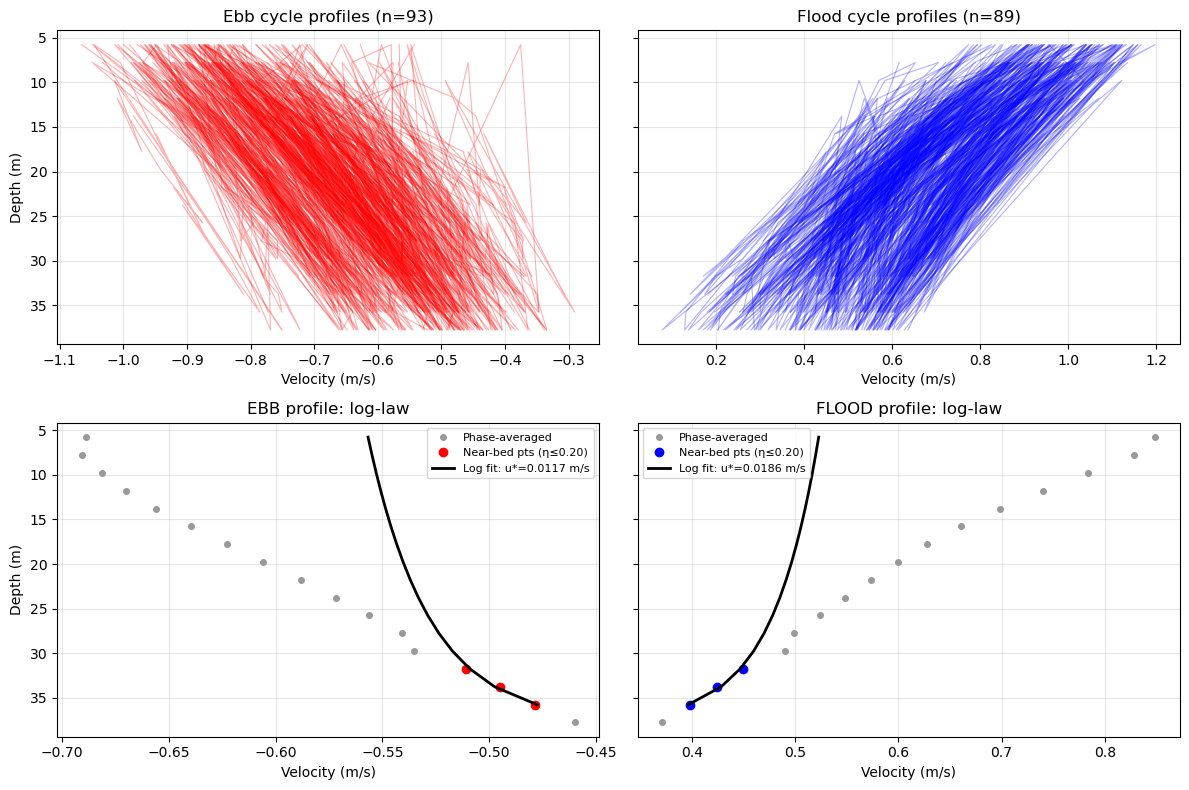
\includegraphics[width=0.85\textwidth]{./figure/log.png} 
  \caption{Representative von K\'arm\'an--Prandtl logarithmic velocity profile illustrating the theoretical near-bed behavior of turbulent boundary-layer flows. The logarithmic formulation is commonly used to describe velocity variation within the inner region of open-channel and tidal boundary layers.}
  \label{Fig:logLaw}
\end{figure}

\begin{figure} [H]
  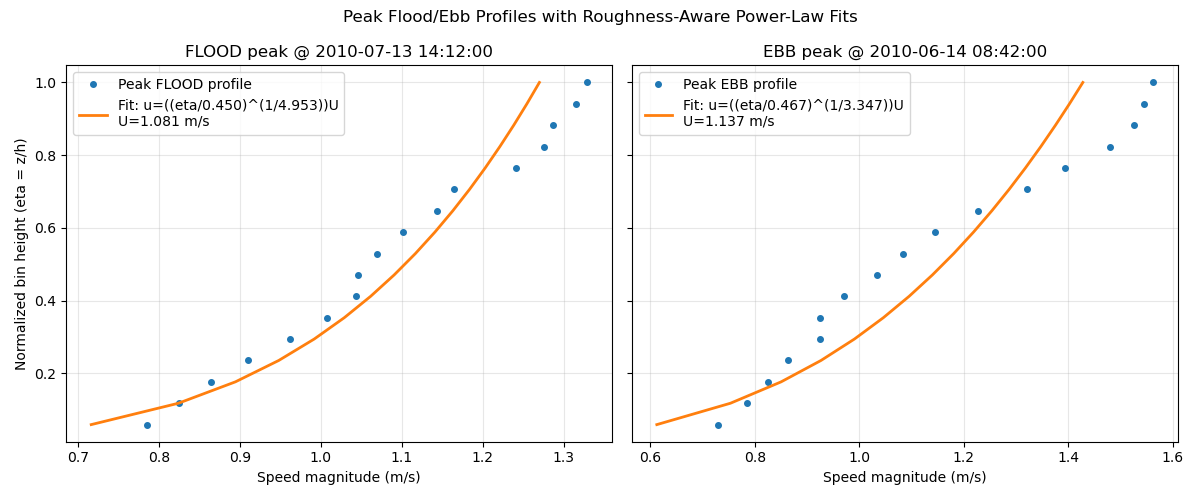
\includegraphics[width=1\textwidth]{./figure/PL.png} 
  \caption{Peak flood and ebb velocity profiles obtained from the Verdant Power ADCP measurements together with the corresponding roughness-aware power-law fits. Blue markers represent measured velocity magnitudes at different normalized elevations, while the orange curves denote the fitted power-law profiles. The fitted parameters indicate slight asymmetry between flood and ebb tidal conditions.}
  \label{Fig:powerLaw}
\end{figure}

\begin{table}[H]
\centering
\caption{H}
\label{tab:fit_stats}
\begin{tabular}{cccc}
\hline
\textbf{Fit} & \textbf{Tide} & \textbf{$R^{2}$ [\%]} & \textbf{$p$} \\
\hline
Cosine & Both & 99.9 & 8.13e-285 \\
Power & Ebb & 94.1 & 1.76e-008 \\
Power & Flood & 97.1 & 9.96e-011 \\ 
Log & Ebb &  &  \\
Log & Flood &  &  \\
\hline
\end{tabular}
\end{table}

\iffalse
\begin{figure} [H]
  \includegraphics[width=1\textwidth]{} 
  \caption{.}
  \label{}
  \label{}
\end{figure}


\begin{table}[H]
\centering
\caption{}
\label{tab:inlet_bcs}
\begin{tabular}{ccc}
\hline
\textbf{Model} & \textbf{Tidal Type} & \textbf{Inlet B.C.}\\
\hline
FL-Lo & Flood & Logarithmic law Velocity Profile\\ 
FL-SC & Flood & Precursor Straight-Channel Simulation\\
FL-RF & Flood & Precursor River Simulation\\
FL-ROMS & Flood & Oceanic inflow conditions Simulation \\
EB-Lo & Ebb & Logarithmic law Velocity Profile\\
\hline
\end{tabular}
\end{table}
\fi

\subsection{Turbulence Intensity}
\label{sec:4.2}

\begin{figure} [H]
  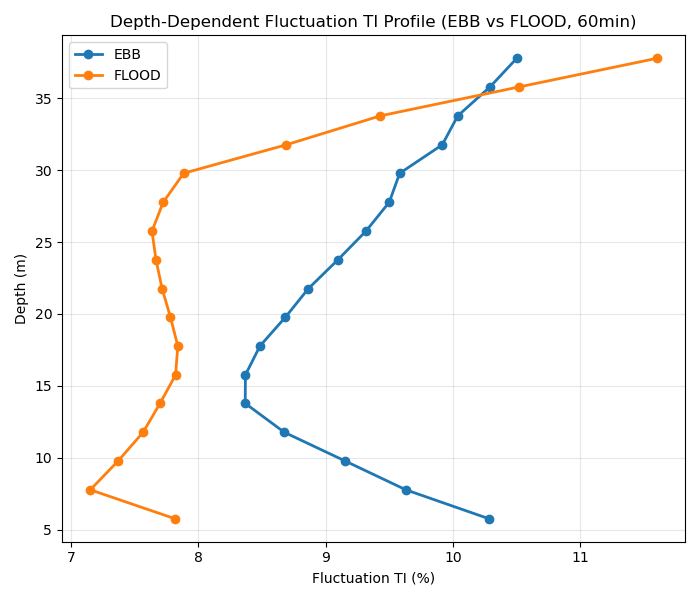
\includegraphics[width=0.65\textwidth]{./figure/TI.png} 
  \caption{Turbulence intensity from phase-averaged depth-dependent velocity data. Depth is given in dimensions of meters.}
  \label{Fig:TI}
\end{figure}

\iffalse
\begin{table}[h!]
\centering
\caption{Tidal conditions selected for comparison between LES results and field measurements.}
\begin{tabular}{lcc}
\hline
\textbf{Tidal Condition} & \textbf{Date} &\textbf{Time (EST)} \\
\hline
Maximum Spring Flood & April 28, 2017 & 11:31 AM \\
Maximum Ebb Tide     & May 1, 2017    & 08:31 AM \\
\hline
\end{tabular}
\label{tab:111}
\end{table}
\fi

\section{Tidal Analysis}

\subsection{Results and Discussion}

\begin{figure} [H]
  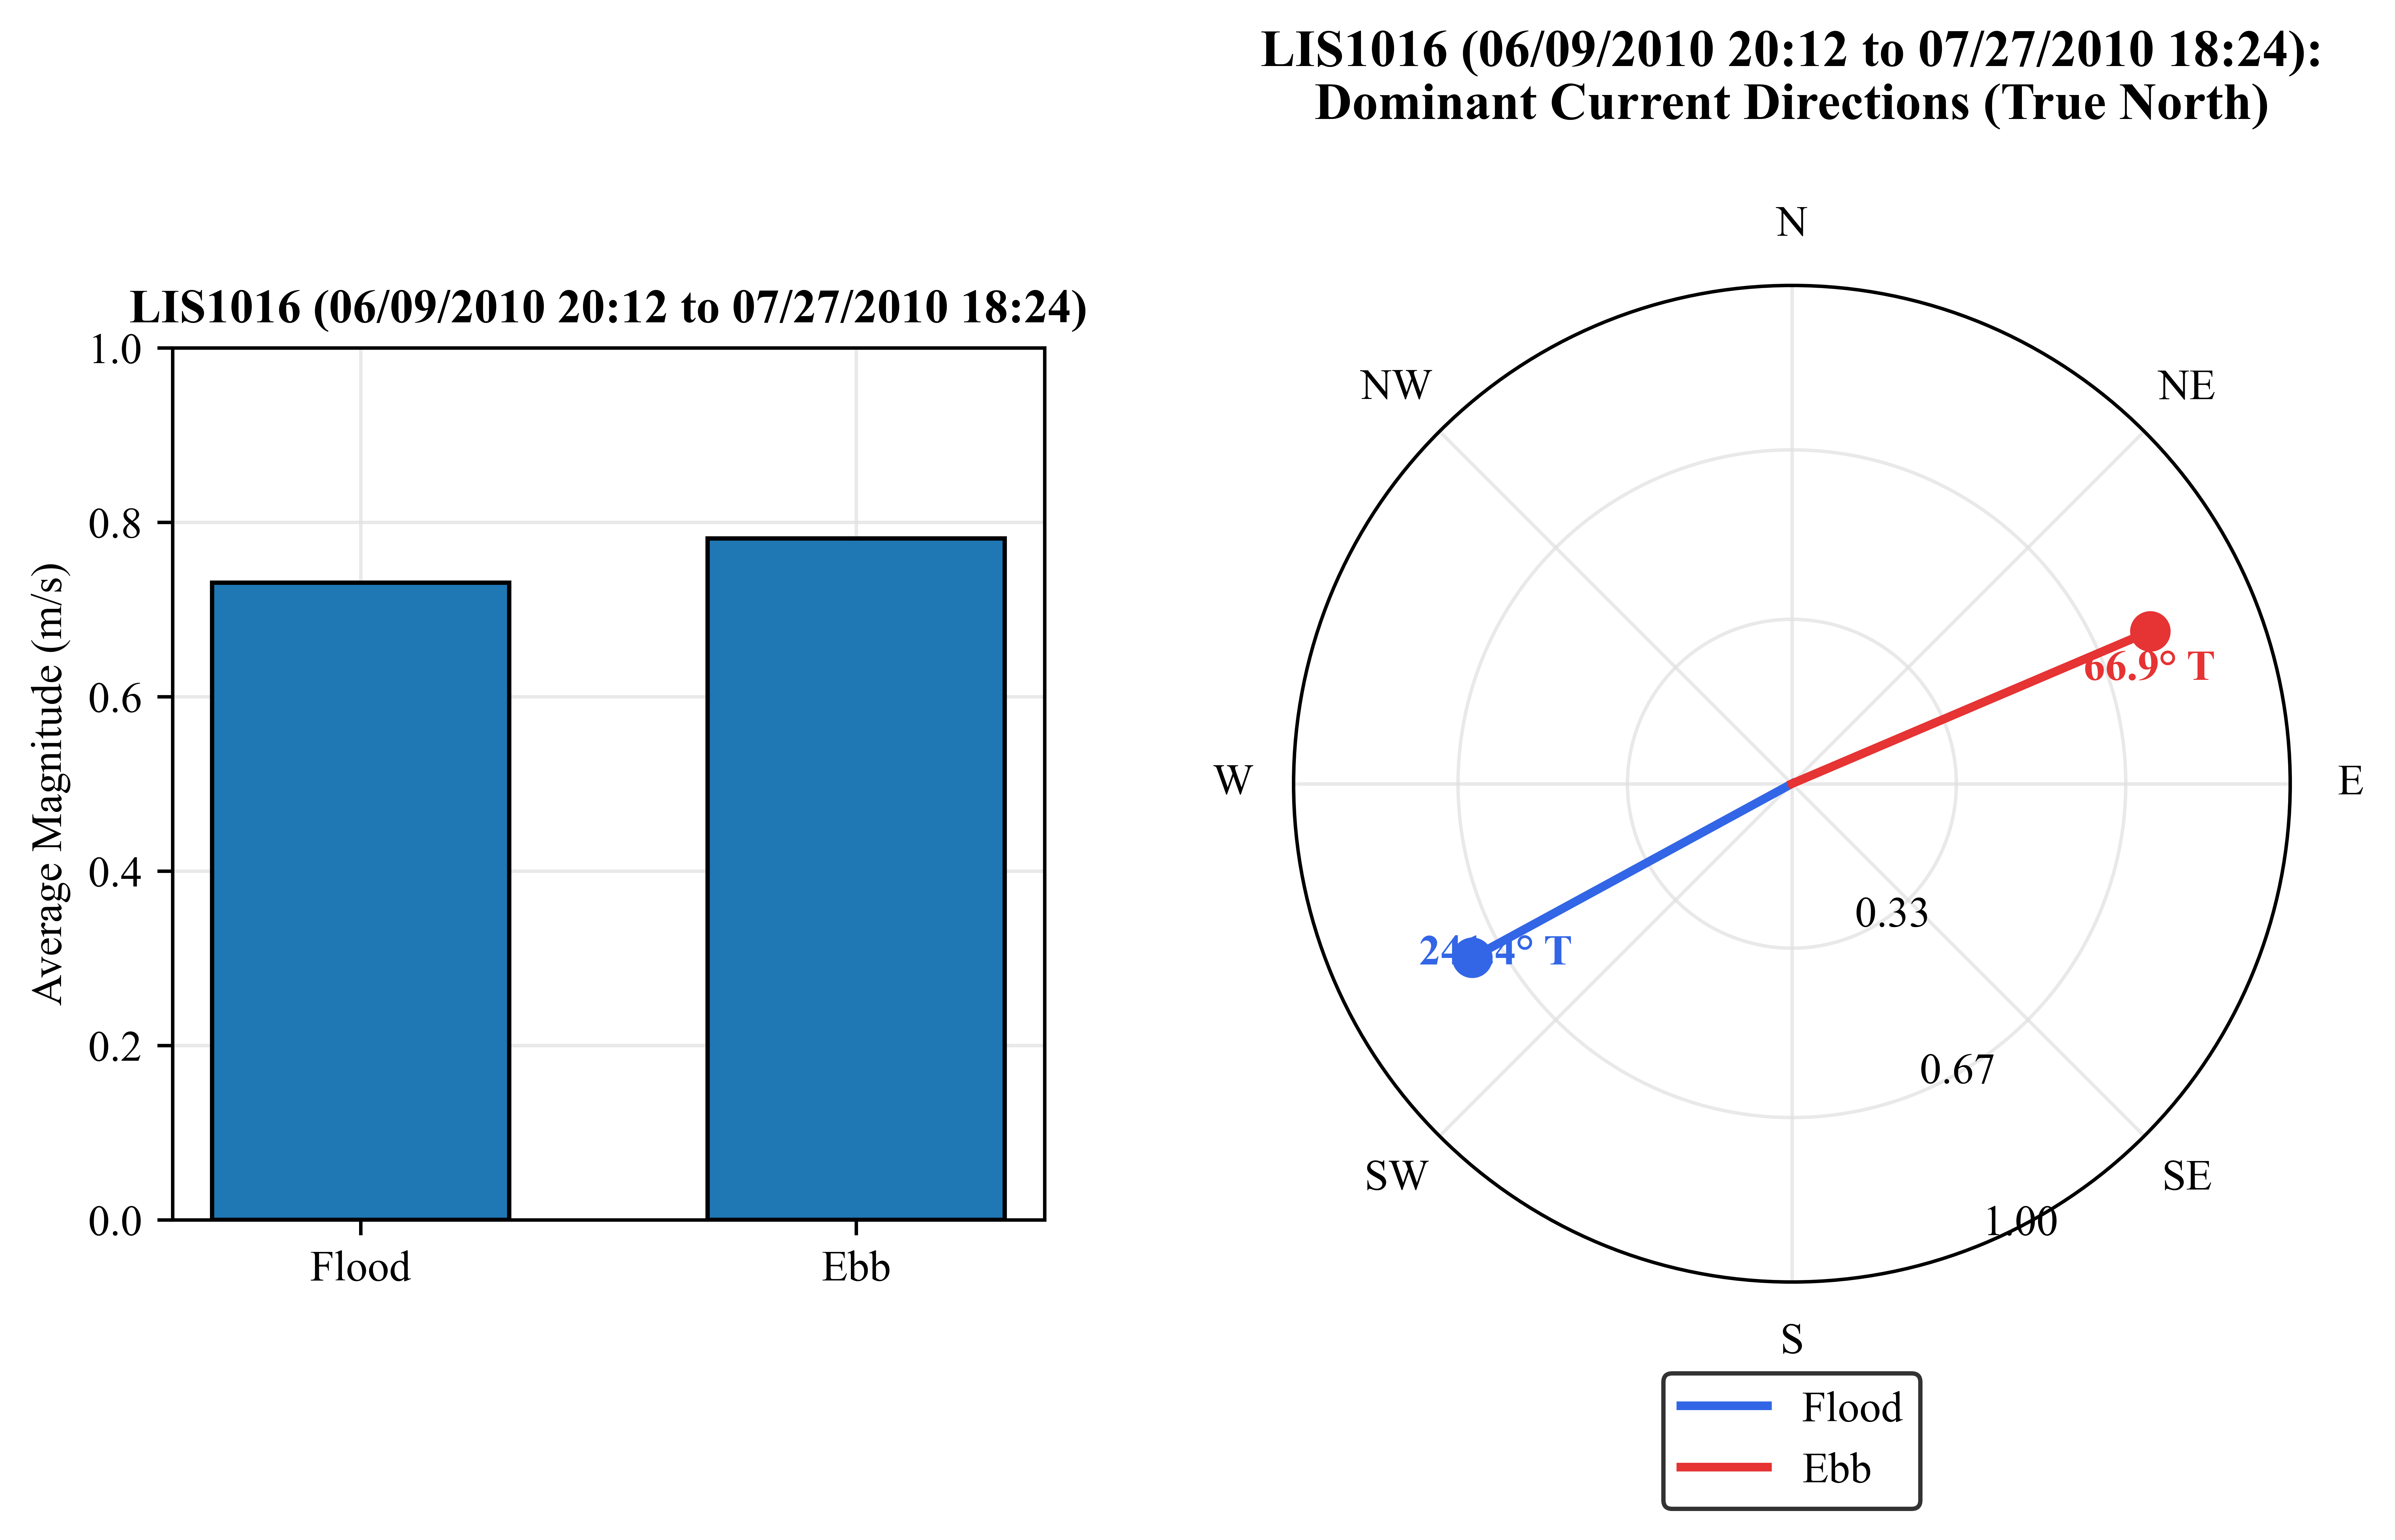
\includegraphics[width=1\textwidth]{./figure/_FlowSummary.png} 
  \caption{The left-hand side displays a histogram of the depth-averaged, time-averaged magnitudes of ebb and flood, which are given in meters per second. The right-hand side displays the compass map of the average dominant directions of tidal current ebb and flood.}
  \label{Fig:flow_summary}
\end{figure}

\begin{figure} [H]
  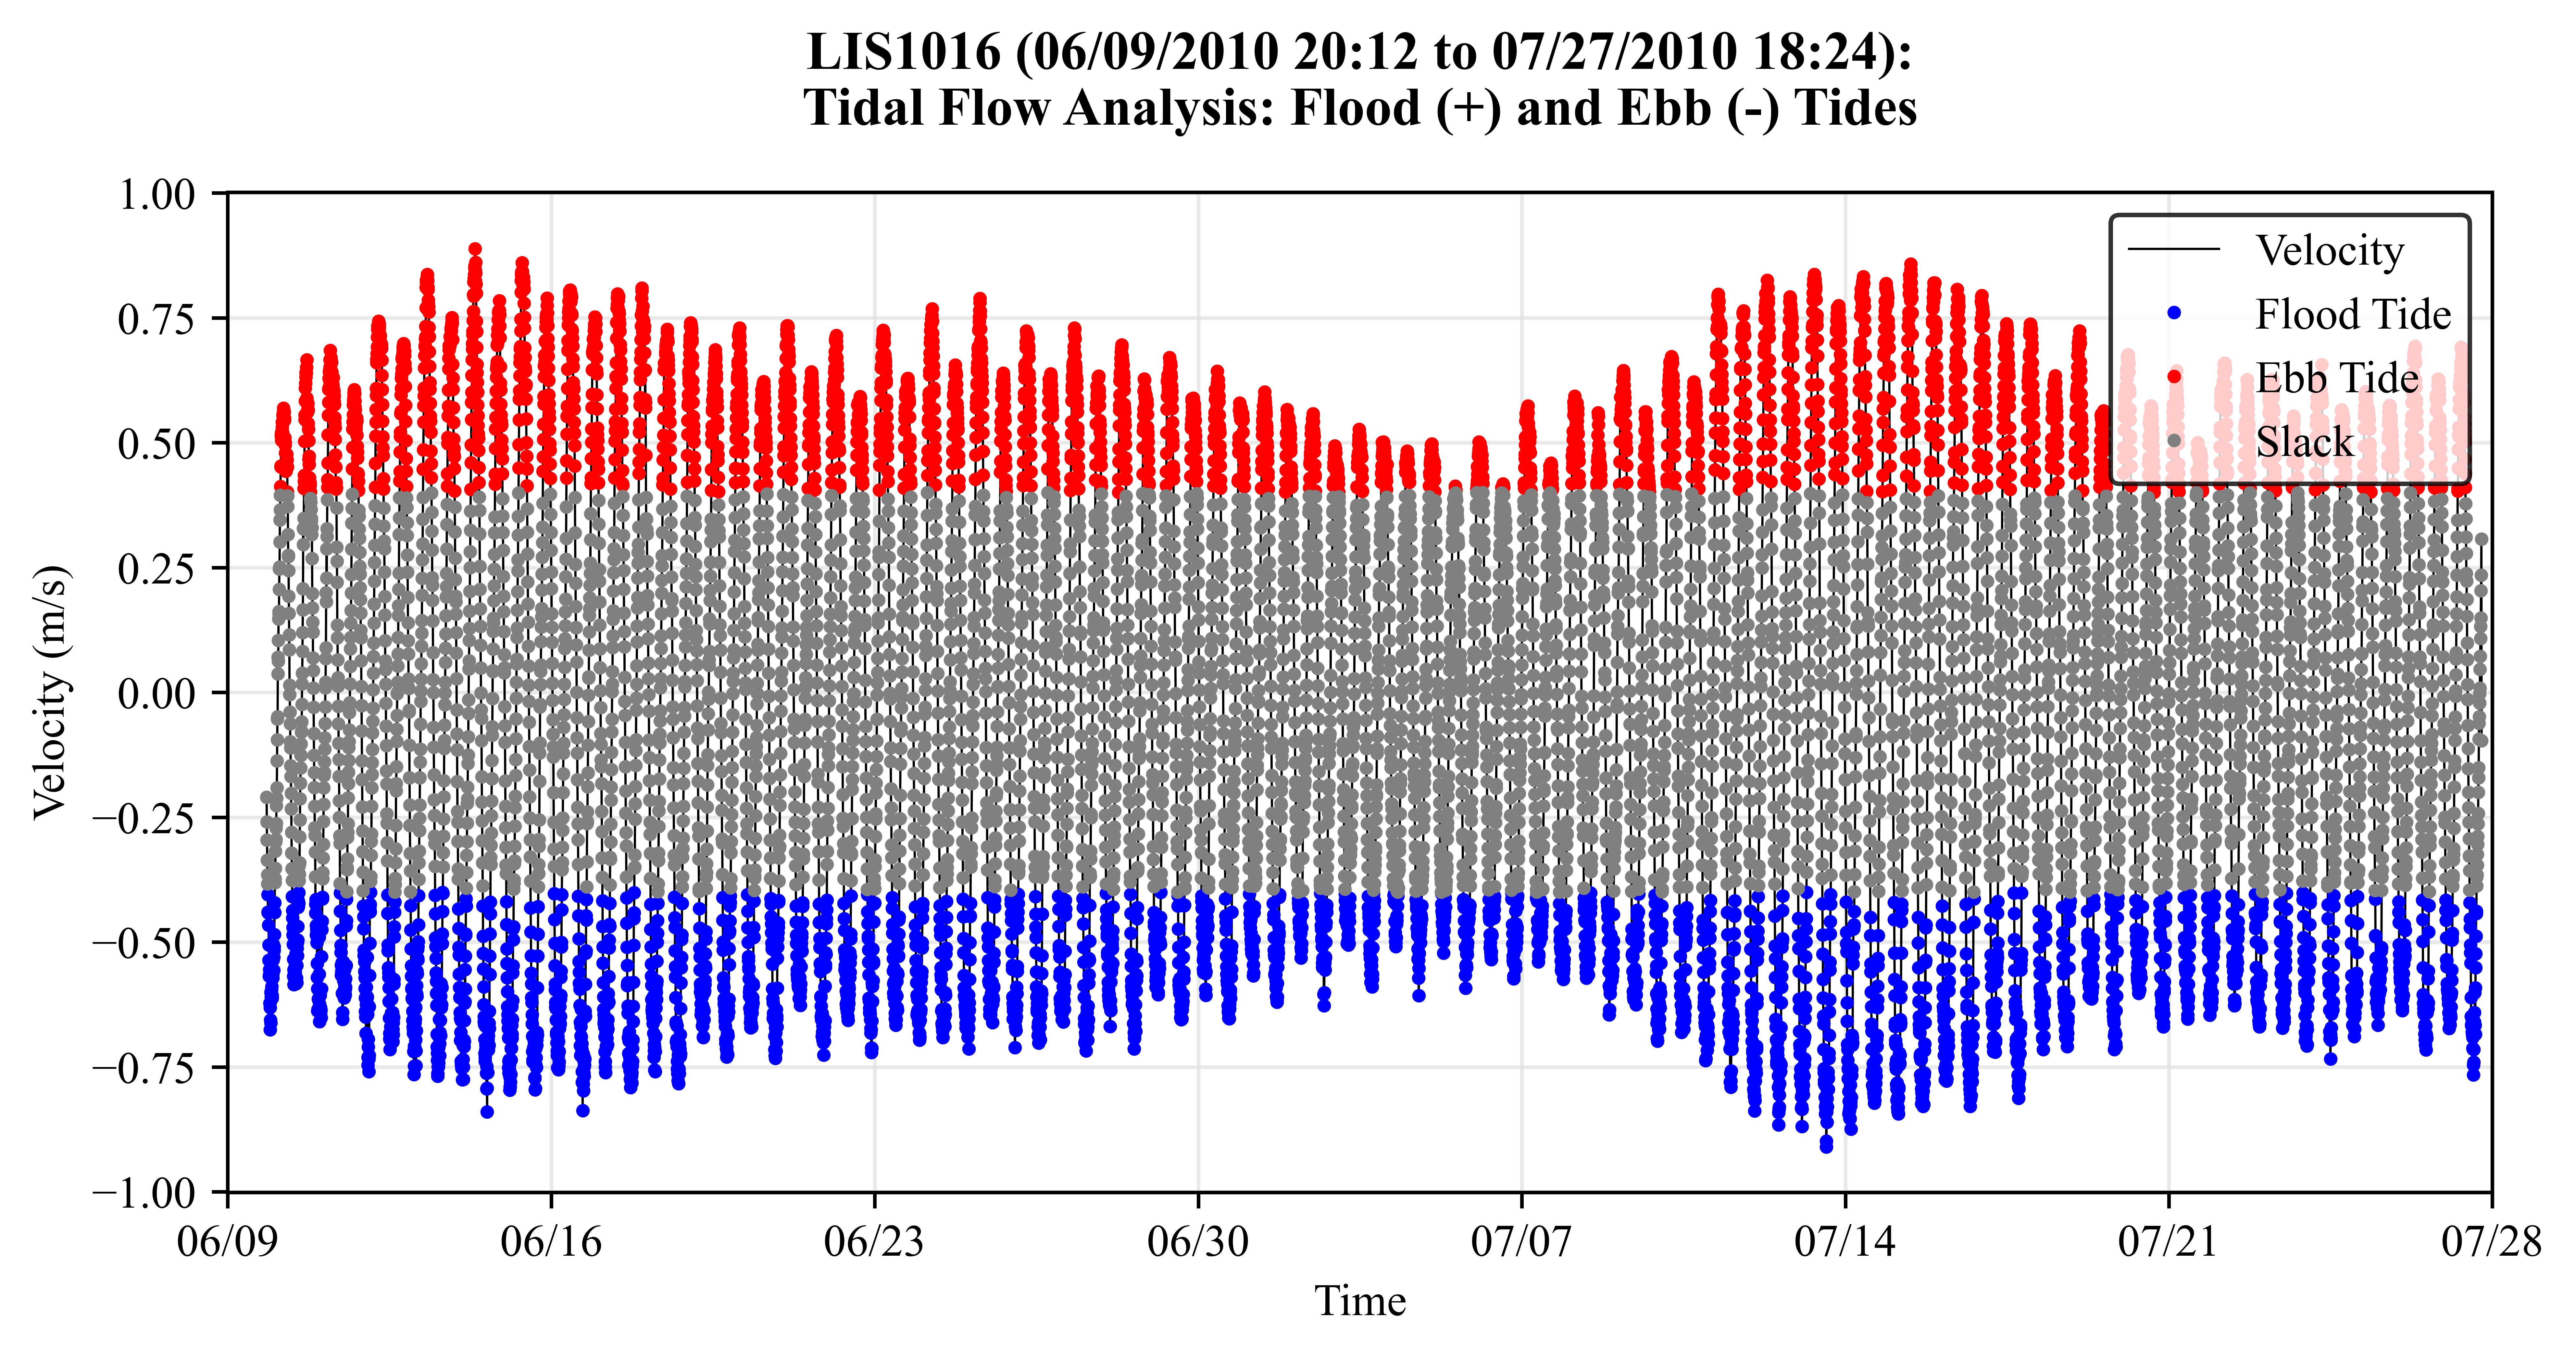
\includegraphics[width=0.75\textwidth]{./figure/_TimeSeries.png} 
  \caption{Red and blue respectively distinguish the data points of depth-averaged ebb and flood in the time-series. Velocity is plotted as a line to visualize the tidal activity.}
  \label{Fig:time_series}
\end{figure}

\begin{figure} [H]
  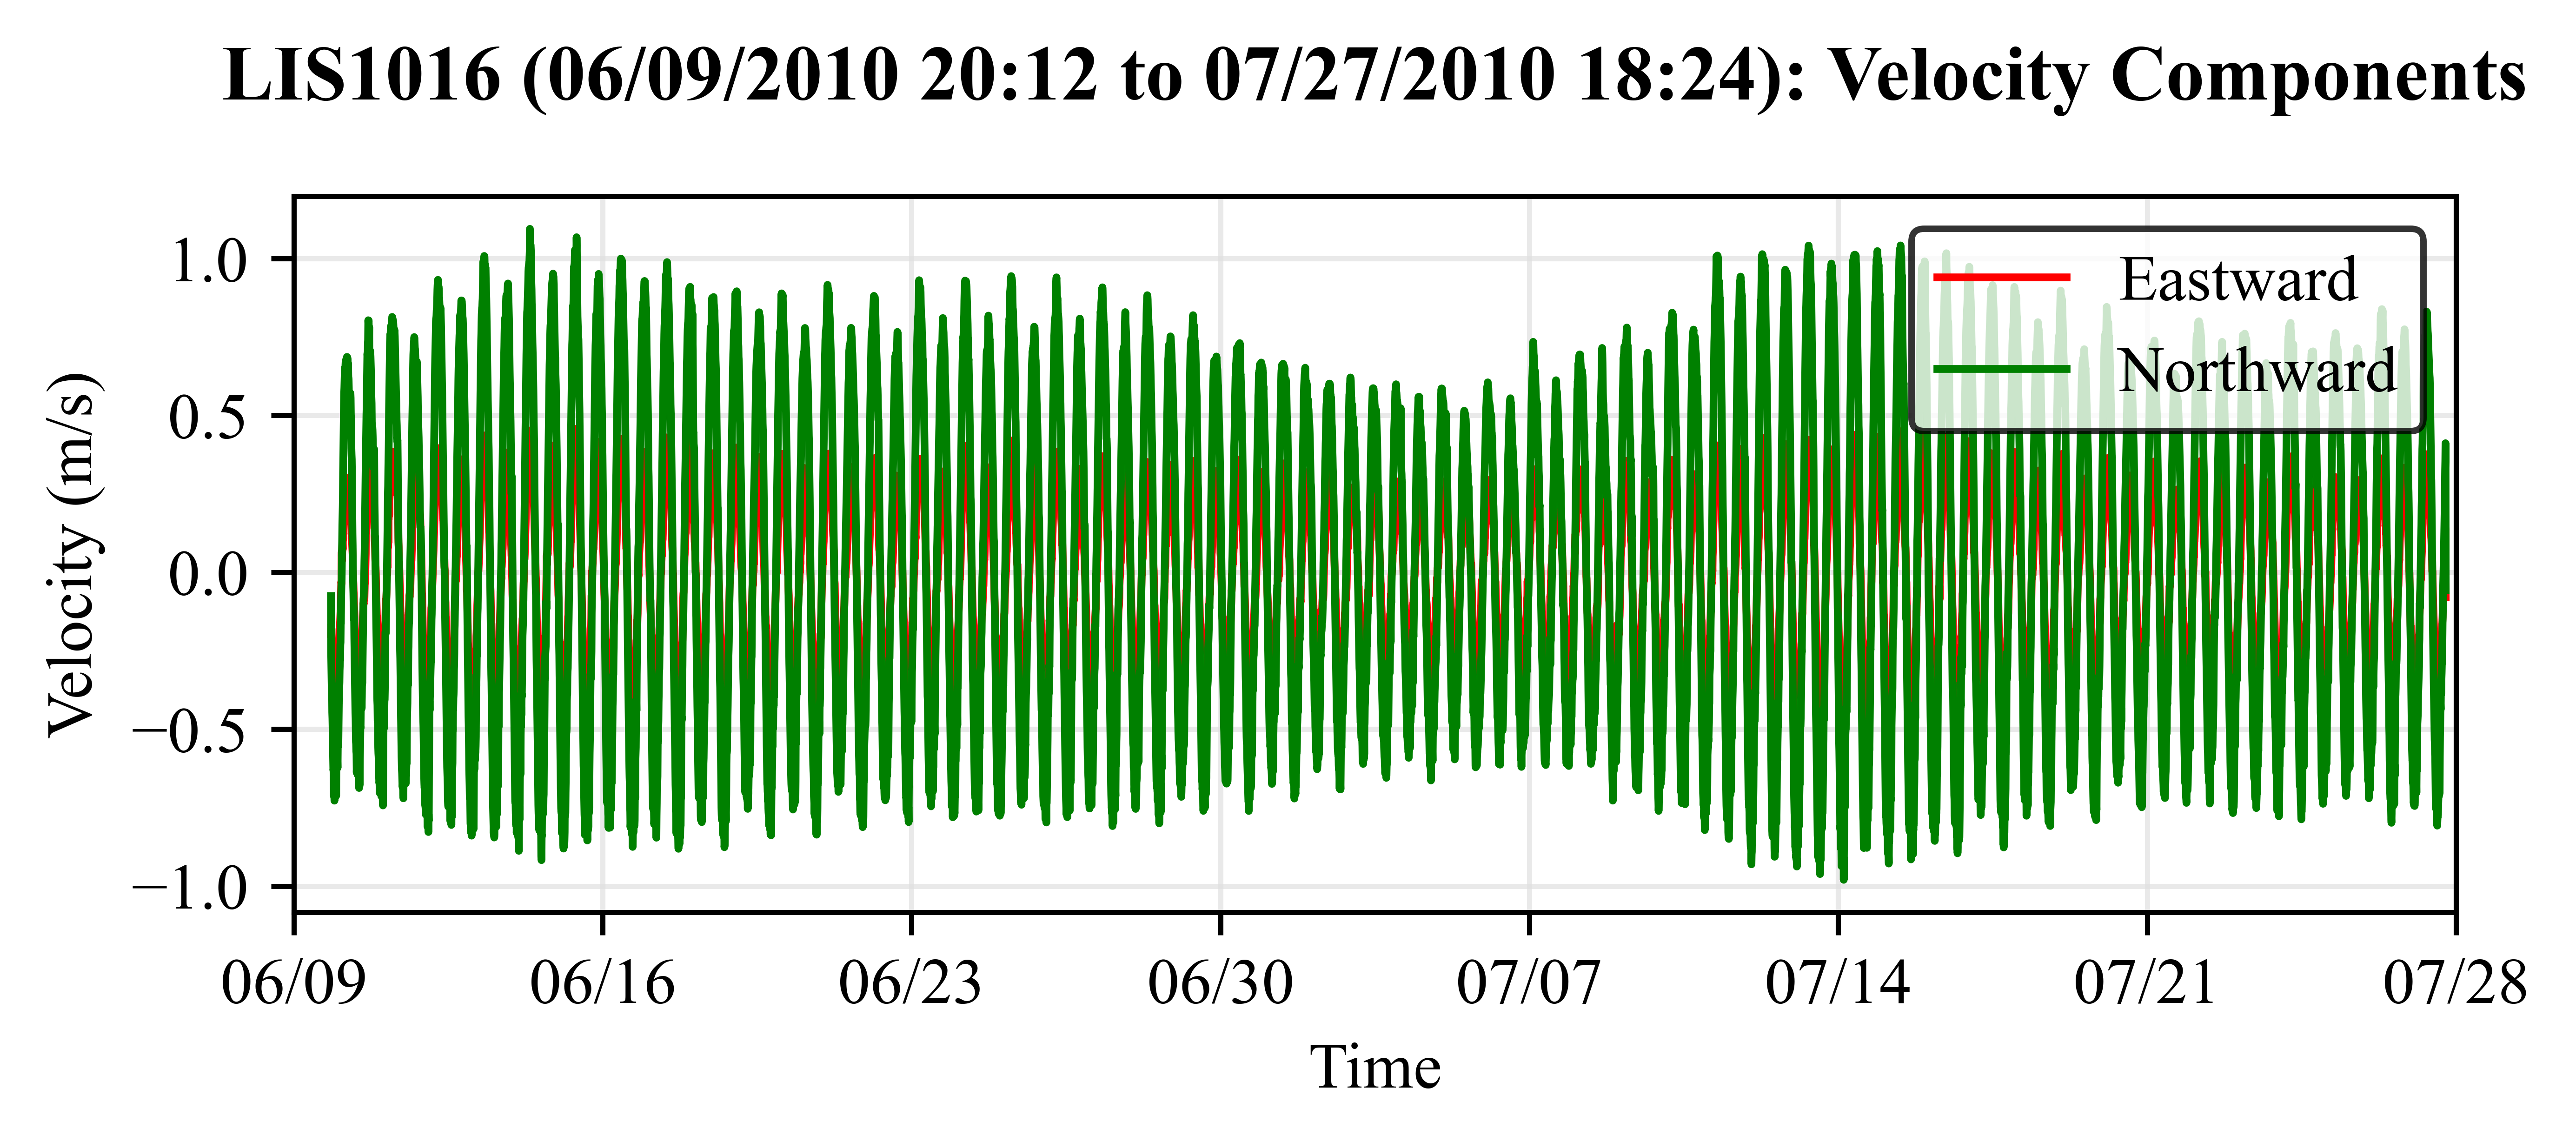
\includegraphics[width=1\textwidth]{./figure/_Components.png} 
  \caption{Tidal velocity is decomposed into northern and eastern components which correspond to green and red, whereby north and east are taken as positive.}
  \label{Fig:velocity_components}
\end{figure}

\begin{figure} [H]
  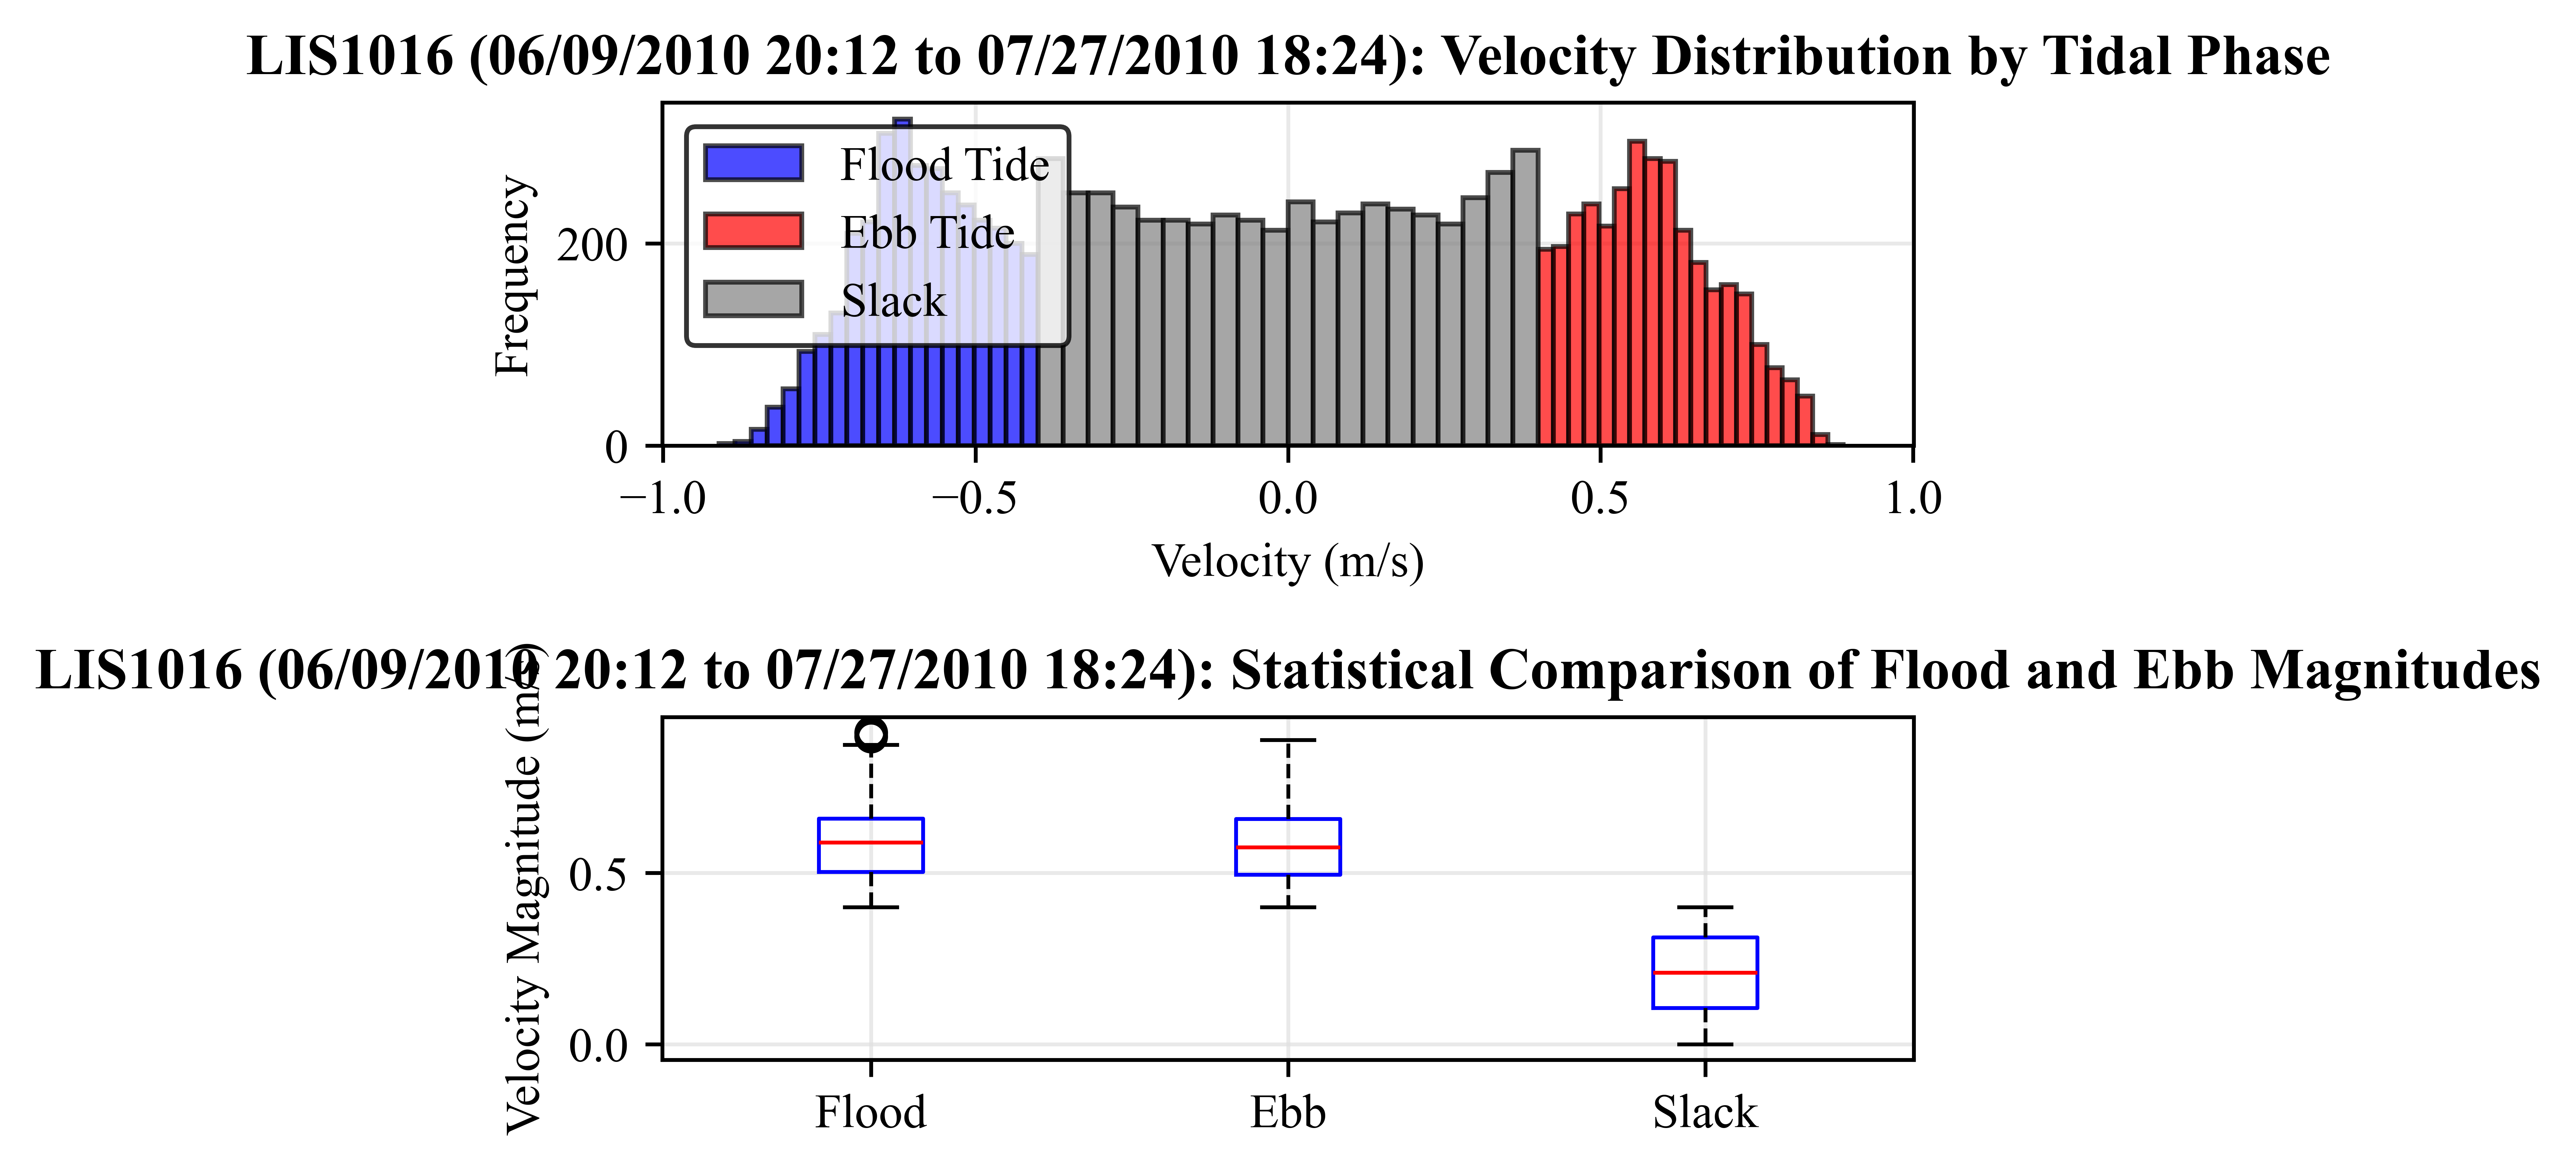
\includegraphics[width=1\textwidth]{./figure/_Statistics.png} 
  \caption{The upper graphic illustrates velocity ranges' frequencies in a histogram of ebb and flood. The lower graphic provides a box plot of both ebb and flood according to velocity.}
  \label{Fig:tide_stats}
\end{figure}

\begin{figure} [H]
  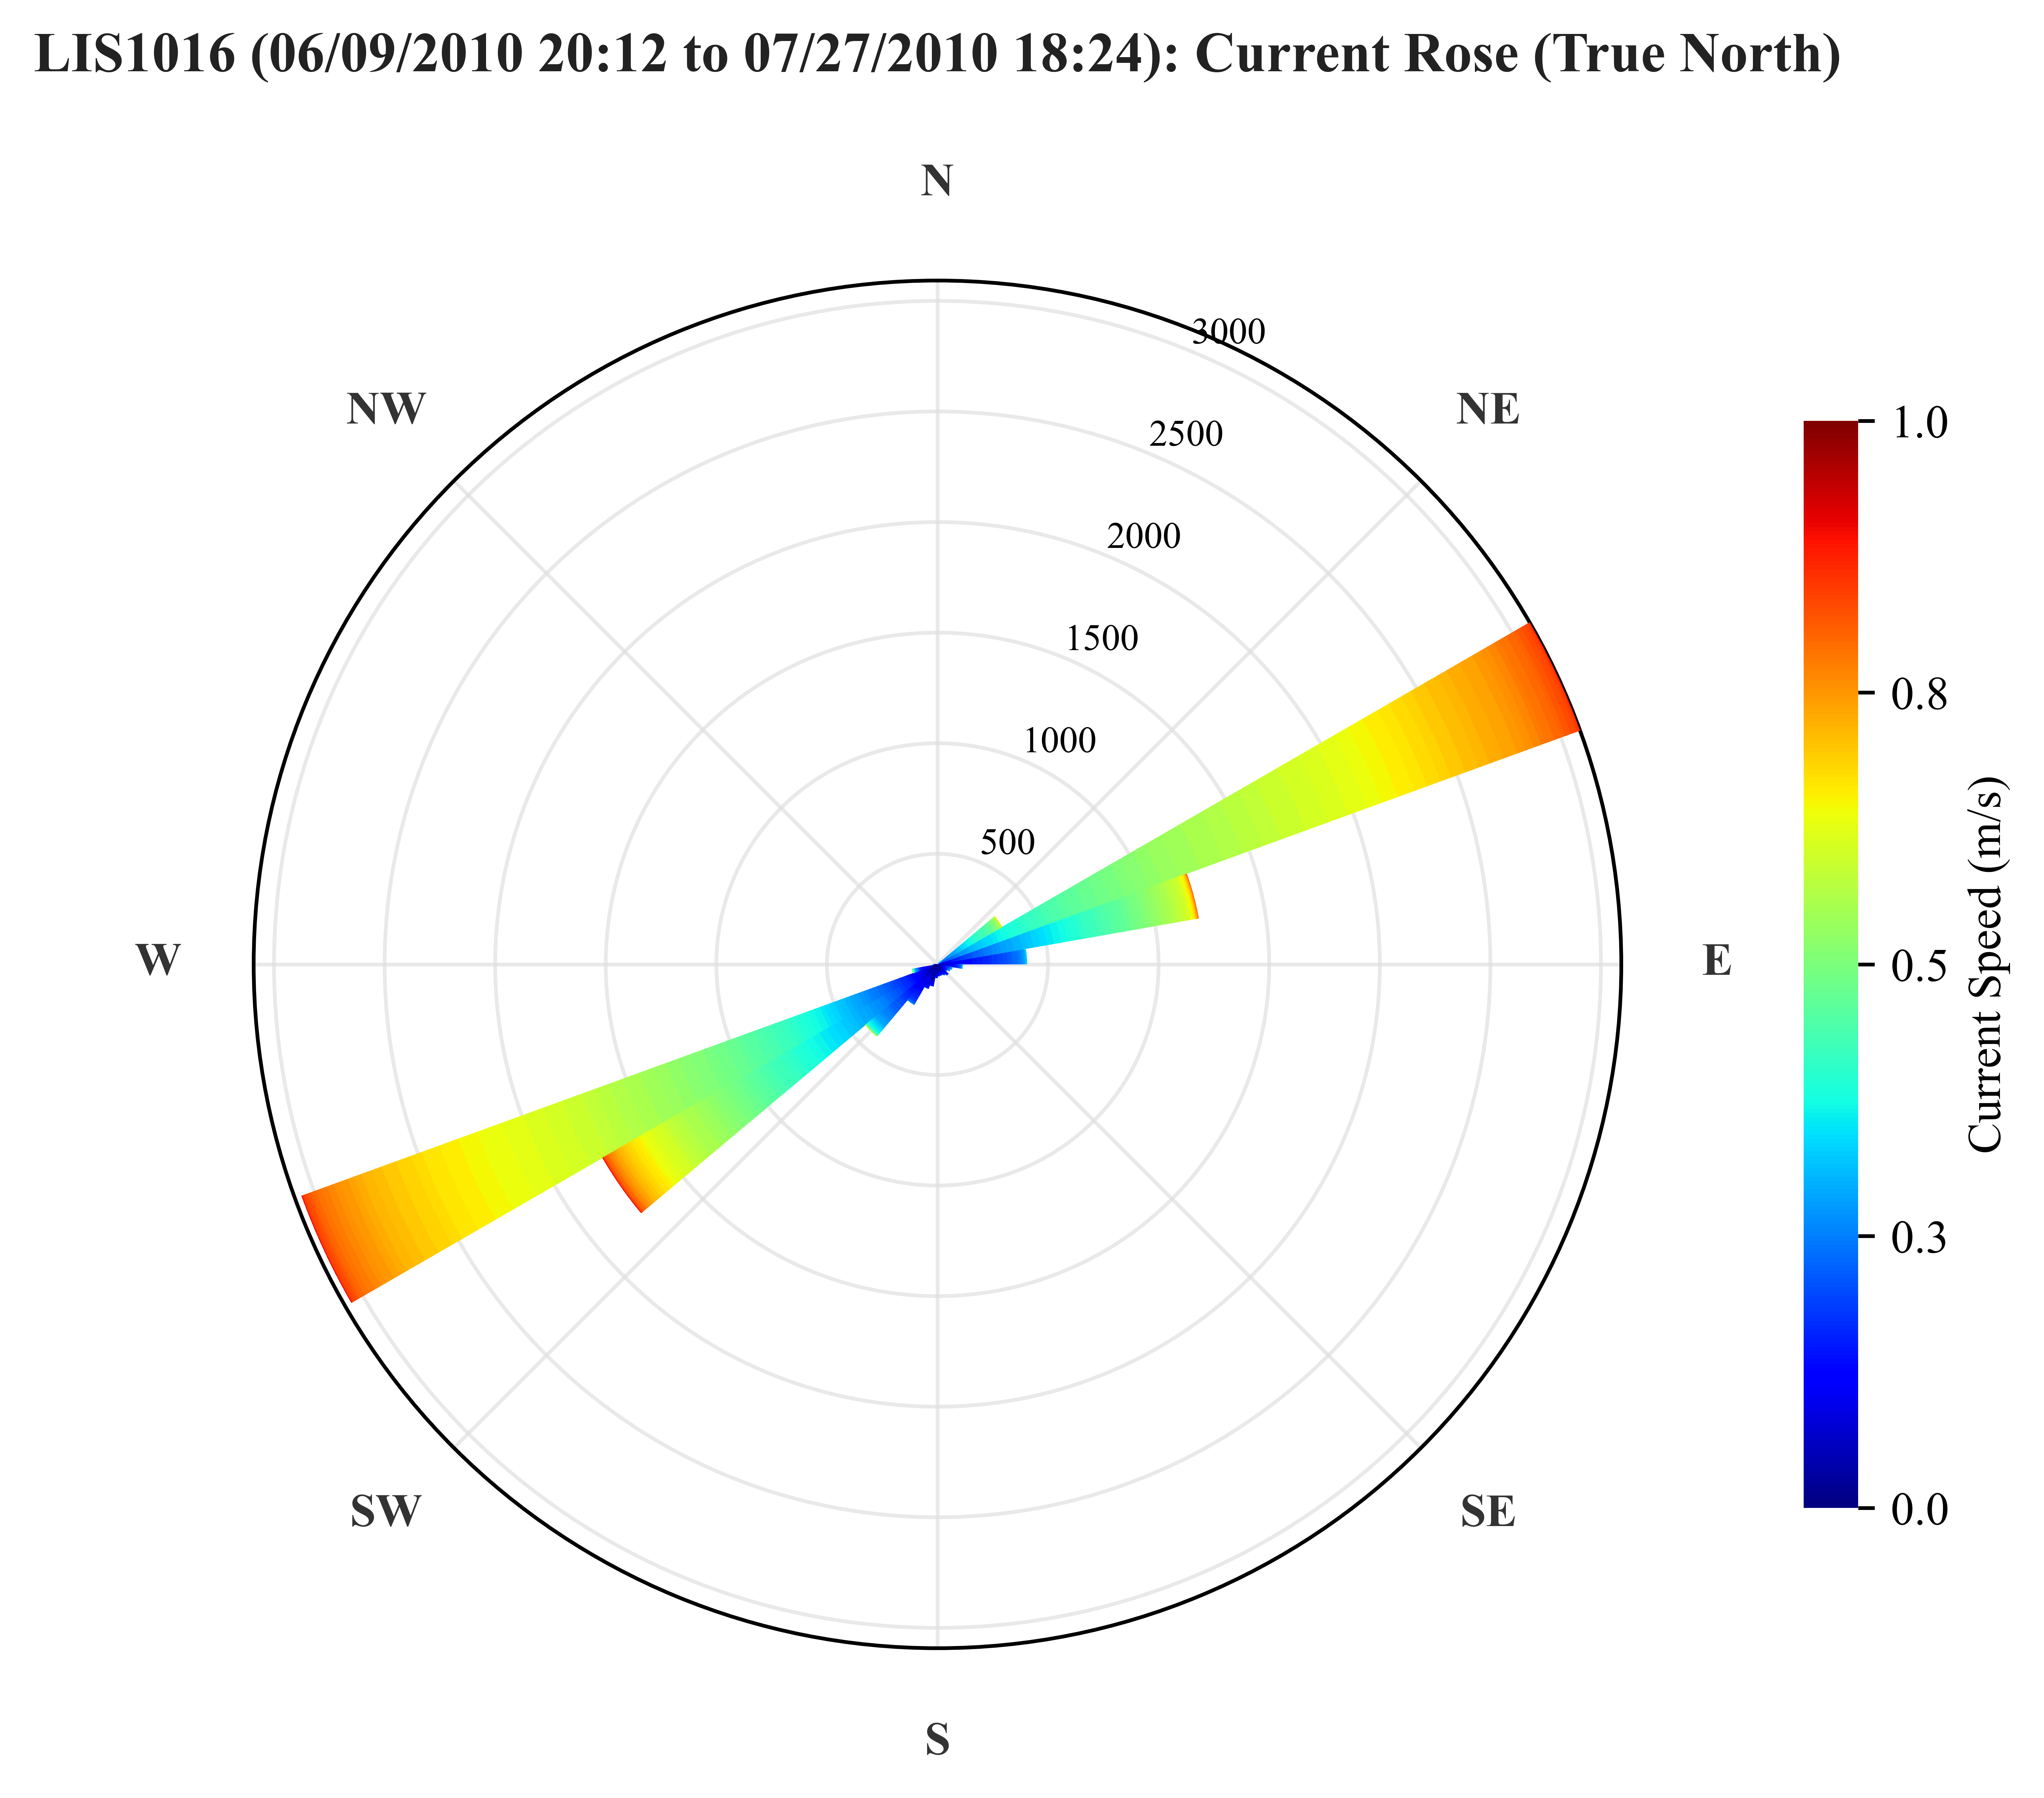
\includegraphics[width=0.5\textwidth]{./figure/_CurrentRose.png} 
  \caption{Set to true north, the current rose visualizes the tidal currents' speeds and directions. The color bar to the right encodes the approximate current speed in meters per second.}
  \label{Fig:current_rose}
\end{figure}

%\begin{figure} [H]
%  \includegraphics[width=1\textwidth]{example-image.png} 
%  \caption{}
%  \label{}
%  \label{}
%\end{figure}

\section{Conclusion}
\label{sec:5}



\section{Acknowledgements}
\label{sec:acknowledge}
\noindent This study is supported by Verdant Power Inc. Also, partial support is provided by the U.S. Department of Energy's Hydropower and Hydrokinetic Office (H2O), under Office of Critical Minerals and Energy Innovation, Award No. DE-EE0009450. The views expressed herein do not necessarily represent the views of the U.S. Department of Energy or the United States Government.

\section{Data Availability Statement} 
\label{sec:7} 

%\appendix
%\section{Grid Sensitivity}
%\label{sec:AppA}

\begin{table} [H]
  \caption{}
  \begin{tabular} {>{\arraybackslash}p{4cm} >{\arraybackslash}p{3cm} >{\arraybackslash}p{3cm} >{\arraybackslash}p{3cm}}
    
    \bottomrule
  \end{tabular}
  
  \label{tab:4}
\end{table}


\begin{figure} [H]
  %\includegraphics[width=0.8\textwidth]{}  
  \caption{}
  \label{}
  \label{}
\end{figure}

\bibliographystyle{elsarticle-num-names} 
\bibliography{main}
\end{document}
%%\endinput
%%
%% End of file `elsarticle-template-num-names.tex'.

